\chapter{Project Design}
The importance of requirement analysis, system design, which includes context and data flow diagrams, as well as project planning and task assignments for this research is stressed in this chapter.

\section{Requirement Analysis}
\subsection{Functional and Nonfunctional Requirements}
\subsubsection{Functional Requirements}
\begin{itemize}
    \item The system must be capable of detecting programmer anxiety through behavioral and contextual clues.
    \item The system must be capable of delivering adaptive interventions in the context of VS Code and Code::Blocks 20.03.
    \item The extension and plugin must be capable of logging events related to programmer anxiety.
    \item The system must be capable of protecting the privacy of the user.
\end{itemize}

\subsubsection{Nonfunctional Requirements}
\begin{itemize}
    \item \textbf{Performance:} The system should have the ability to detect threats and perform countermeasures at the maximum speed.
    \item \textbf{Usability:} The extension and plugin should occupy minimal space when installing, and it should not hinder the coding process of the programmer.
    \item \textbf{Scalability:} The system should be able to run several programming classes and accommodate many users at the same time.
    \item \textbf{Security:} The data that will be collected should be private and anonymous.
\end{itemize}

\subsection{Context Diagram}
We illustrate the interaction between the proposed anxiety detection system and the outer environment through the use of a context diagram. The central component of our system includes the VS Code extension and Code::Blocks 20.03 plugin responsible for the collection of data from the Programmer User, including File Keystrokes, File Active m/s, Keystrokes Total, Active m/s Total, Idle m/s Total, Avg Key m/s, Undo Count, Redo Count, Compile Attempts, JS Errors, eye tracking data including blink rate and fixation patterns. In addition to that, the system can collect data from the Coding Environment IDE, which includes environment events and contextual Information.

We illustrate a closed loop feedback system, with the extension being the main component responsible for data collection. Data collected by the extension is transferred to the Anxiety Detection Engine for analysis purposes; as a result, analysis results are provided to the Anxiety Alert and Recommendation System, and finally data and events are recorded in Database Logs.

\begin{figure}[h]
    \centering
    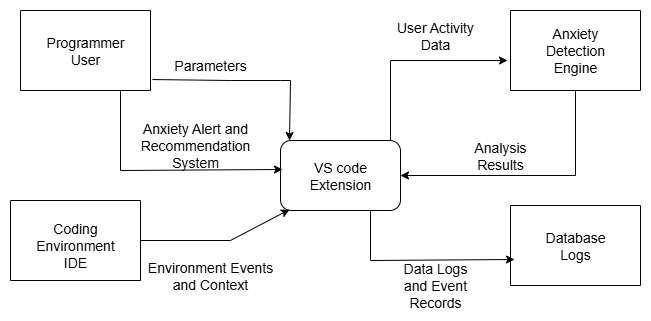
\includegraphics[width=0.8\textwidth]{Context1.png}
    \caption{Context Diagram of the Proposed System}
    \label{fig:context-diagram}
\end{figure}

\subsection{Data Flow Diagram}
It should be noted that the suggested approaches to the development of real-time anxiety detection are quite consistent with current findings in the area of programming education, psychological monitoring, and machine learning. The research shows that programming can become more motivational and stress-free when AI techniques are involved \cite{stemedu2025, programmingAnxiety2025}. Emotional states can be predicted through the use of behavioral data like keystrokes \cite{keystroke2023, realtimeStress2012}. The use of automated sensing combined with self-reporting leads to the most accurate results \cite{mdpi5739}. However, so far, no system has been developed that combines the real-time detection and mitigation of anxiety in an IDE. Such research gap might help develop useful systems.

According to Figure \ref{fig:dfd}, there is a breakdown of the overall system architecture into various modules. The system architecture suggests that the programmer activities will be captured by the Capture Input module both from the Programmer and the IDE environments. The user inputs will be captured using keystrokes, logs, and behavioral data. This module enables the system to detect anxiety from the users' inputs through the Detect Anxiety module. This will be done through provision of feedback to the users, including logging data through the Intervene module. The system would use the Log Data module to capture data collected from results of the system interventions.

\begin{figure}[h]
    \centering
    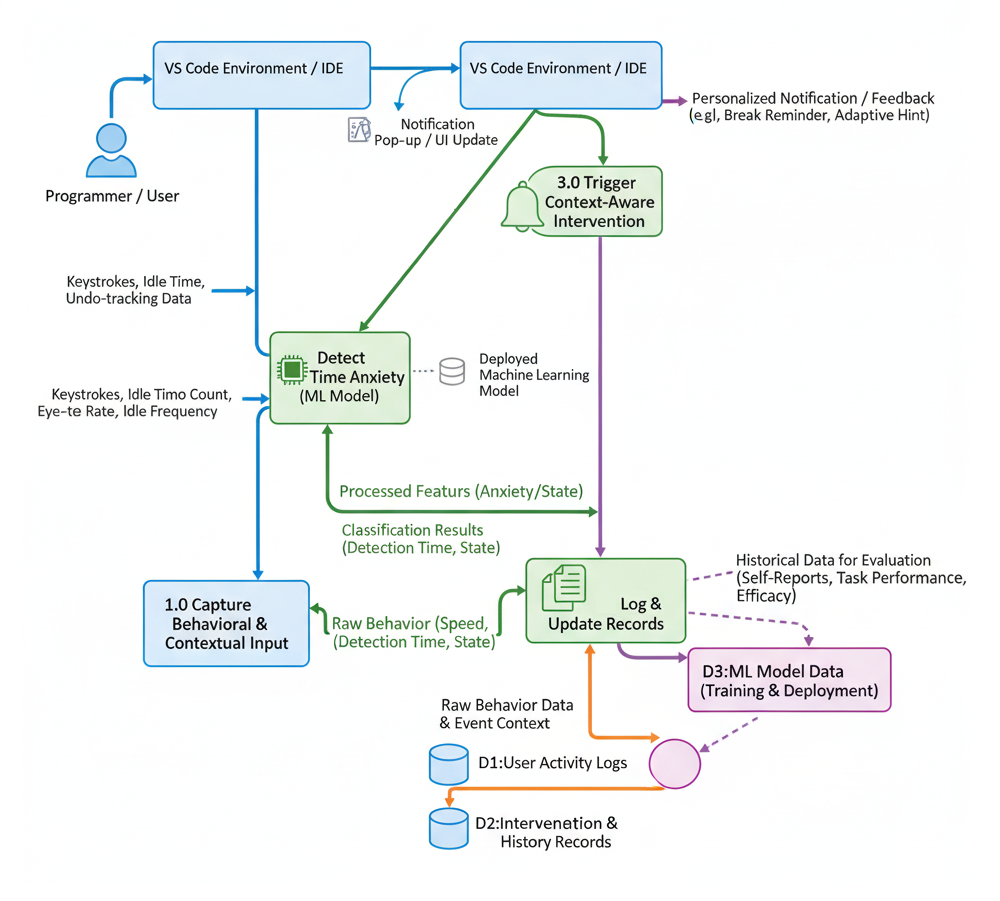
\includegraphics[width=0.8\textwidth]{Dataflow_Diagram_2.png}
    \caption{Data Flow Diagram of the Proposed System}
    \label{fig:dfd}
\end{figure}

\subsection{UI Design}
User Interface design is aimed at awareness and accessibility. As can be seen in Figure \ref{fig:ui-design}, the "Anxiety Copilot" side panel will give a summary of the current state of the user, providing the current level of anxiety as well as the current state of the user's focus. This UI design has the intervention history, which will serve the purpose of reflection by the developers regarding any stress factors. A very important part of the UI design is the notification toast that suggests a mindful activity or a breathing practice.

\begin{figure}[h]
    \centering
    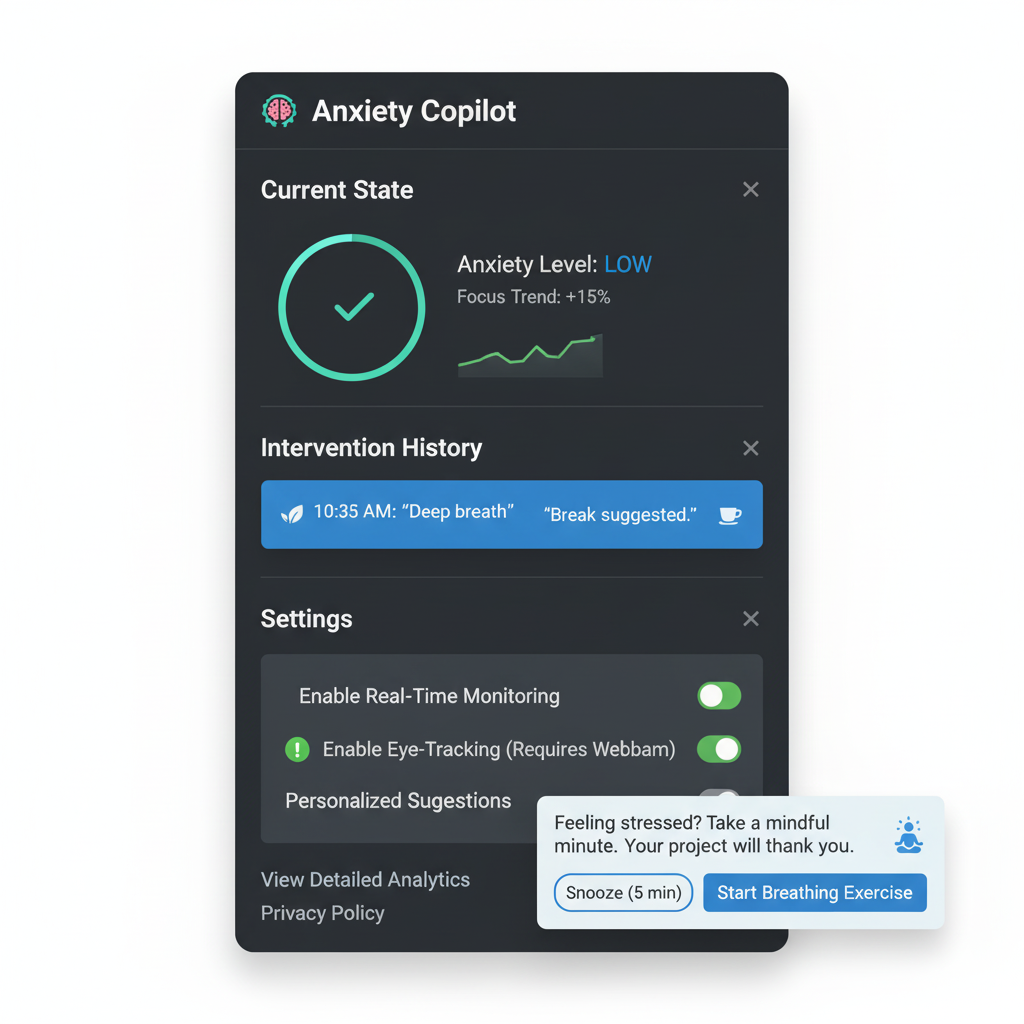
\includegraphics[width=0.9\textwidth]{UI Design.png}
    \caption{Proposed User Interface Design for the Extension}
    \label{fig:ui-design}
\end{figure}